% ============================================================
%  SANJEEVANI — PITCH DECK
%  LaTeX Beamer 16:9, pdfLaTeX-compatible
%  Compile: pdflatex main.tex
% ============================================================
\documentclass[aspectratio=169,t]{beamer}

% ── packages ──────────────────────────────────────────────
\usepackage[utf8]{inputenc}
\usepackage[T1]{fontenc}
\usepackage{lmodern}
\usepackage{tikz}
\usetikzlibrary{shapes.geometric,arrows.meta,positioning,fit,
                backgrounds,calc,matrix}
\usepackage{booktabs}
\usepackage{array}
\usepackage{colortbl}
\usepackage{xcolor}
\usepackage{microtype}
\usepackage{hyperref}

% ── page geometry & margins ────────────────────────────────
\setbeamersize{text margin left=7mm,text margin right=7mm}

% ── colour palette ─────────────────────────────────────────
\definecolor{NavyBg}          {HTML}{08121E}  % Deep Midnight Navy
\definecolor{NavySurface}     {HTML}{112238}  % Elevated Card Surface
\definecolor{NavySurfaceLight}{HTML}{1A3250}  % Card inner accent
\definecolor{NavyBorder}      {HTML}{24456B}  % Card subtle border
\definecolor{Teal}            {HTML}{0FA3B1}  % Primary Accent
\definecolor{TealLight}       {HTML}{4DD8E6}  % High-contrast readable teal
\definecolor{TealDark}        {HTML}{0A4A54}  % Pill fill
\definecolor{Orange}          {HTML}{F58220}  % Warning / Attention
\definecolor{OrangeLight}     {HTML}{FDBA74}  % High-contrast readable orange
\definecolor{OrangeDark}      {HTML}{522406}  % Warning pill fill
\definecolor{Green}           {HTML}{10B981}  % Success / Verified
\definecolor{GreenLight}      {HTML}{6EE7B7}  % High-contrast readable green
\definecolor{GreenDark}       {HTML}{064E3B}  % Success pill fill
\definecolor{Red}             {HTML}{EF4444}  % Alert / Misalignment
\definecolor{RedLight}        {HTML}{FCA5A5}  % High-contrast readable red
\definecolor{TextMain}        {HTML}{F8FAFC}  % Crisp off-white body text
\definecolor{TextMuted}       {HTML}{94A3B8}  % Slate 400 for subtitles/captions
\definecolor{TextSub}         {HTML}{CBD5E1}  % Slate 300 for readable descriptions
\definecolor{GoldStar}        {HTML}{FBBF24}  % Amber highlight

% ── Beamer theme ───────────────────────────────────────────
\usetheme{default}
\usecolortheme{default}
\setbeamercolor{background canvas}    {bg=NavyBg}
\setbeamercolor{normal text}          {fg=TextMain,bg=NavyBg}
\setbeamercolor{frametitle}           {fg=TealLight,bg=NavyBg}
\setbeamercolor{framesubtitle}        {fg=TextMuted}
\setbeamercolor{itemize item}         {fg=TealLight}
\setbeamercolor{itemize subitem}      {fg=Teal}
\setbeamercolor{enumerate item}       {fg=TealLight}
\setbeamercolor{alerted text}         {fg=OrangeLight}
\setbeamercolor{footer}               {fg=TextMuted}

\setbeamertemplate{navigation symbols}{}
\setbeamertemplate{itemize item}{\scriptsize\raisebox{0.5pt}{\textcolor{TealLight}{$\blacktriangleright$}}}
\setbeamertemplate{itemize subitem}{\tiny\raisebox{0.5pt}{\textcolor{Teal}{$\circ$}}}

\setbeamerfont{frametitle}{size=\large,series=\bfseries}
\setbeamerfont{framesubtitle}{size=\scriptsize}

% Custom frametitle template with precise spacing
\setbeamertemplate{frametitle}{%
  \vspace{0.16cm}%
  \begin{beamercolorbox}[wd=\paperwidth,leftskip=7mm,rightskip=7mm]{frametitle}
    {\usebeamerfont{frametitle}\color{TealLight}\insertframetitle\par}%
    \ifx\insertframesubtitle\@empty%
    \else%
      \vspace{1pt}%
      {\usebeamerfont{framesubtitle}\color{TextMuted}\insertframesubtitle\par}%
    \fi%
  \end{beamercolorbox}%
  \vspace{-0.22cm}%
}

% Custom footer template
\setbeamertemplate{footline}{%
  \begin{beamercolorbox}[wd=\paperwidth,ht=2.5ex,dp=1.0ex,leftskip=7mm,rightskip=7mm]{footer}
    \scriptsize\color{TextMuted}%
    \textbf{\textcolor{Teal}{SANJEEVANI}} \quad\textbar\quad \textit{Practice before the moment.}%
    \hfill%
    \textcolor{TextMuted}{Android AR Emergency Training} \quad\textbar\quad \textbf{\textcolor{TealLight}{\insertframenumber}}\,/\,\inserttotalframenumber%
  \end{beamercolorbox}%
}

% ── reusable TikZ styles ───────────────────────────────────
\tikzset{
  surface/.style     = {rectangle,rounded corners=4pt,fill=NavySurface,
                        draw=NavyBorder,line width=0.6pt,text=TextMain,
                        inner sep=5pt,align=left},
  tealsurface/.style = {surface,draw=Teal!80},
  orangesurface/.style={surface,draw=Orange!80},
  greensurface/.style= {surface,draw=Green!80},
  subtlebox/.style   = {rectangle,rounded corners=3pt,fill=NavySurfaceLight,
                        draw=NavyBorder!50,line width=0.5pt,text=TextMain,
                        inner sep=3.5pt,align=left},
  pill/.style        = {rectangle,rounded corners=3pt,fill=TealDark,
                        draw=Teal!90,line width=0.6pt,text=TealLight,
                        font=\scriptsize\bfseries,inner sep=3pt},
  orangepill/.style  = {rectangle,rounded corners=3pt,fill=OrangeDark,
                        draw=Orange!90,line width=0.6pt,text=OrangeLight,
                        font=\scriptsize\bfseries,inner sep=3pt},
  greenpill/.style   = {rectangle,rounded corners=3pt,fill=GreenDark,
                        draw=Green!90,line width=0.6pt,text=GreenLight,
                        font=\scriptsize\bfseries,inner sep=3pt},
  arrow/.style       = {-{Stealth[length=4.5pt]},TealLight,line width=1.1pt},
  arrowO/.style      = {-{Stealth[length=4.5pt]},OrangeLight,line width=1.1pt},
  arrowG/.style      = {-{Stealth[length=4.5pt]},GreenLight,line width=1.1pt},
  arrowDashed/.style = {-{Stealth[length=4pt]},TextMuted,line width=0.7pt,dashed},
}

% ── helper commands ────────────────────────────────────────
\newcommand{\teal}[1]{\textcolor{TealLight}{#1}}
\newcommand{\orange}[1]{\textcolor{OrangeLight}{#1}}
\newcommand{\green}[1]{\textcolor{GreenLight}{#1}}
\newcommand{\tsub}[1]{\textcolor{TextMuted}{\footnotesize #1}}
\newcommand{\impl}{\textcolor{GreenLight}{\textbf{[Implemented]}}}
\newcommand{\prop}{\textcolor{OrangeLight}{\textbf{[Proposed]}}}

% ── meta ──────────────────────────────────────────────────
\title{\textbf{SANJEEVANI}}
\subtitle{Practice before the moment.}
\author{Emergency Skills Training Platform}
\date{}

% ===========================================================
\begin{document}

% ── SLIDE 1: COVER ─────────────────────────────────────────
{
\setbeamertemplate{footline}{}
\begin{frame}[plain]
\begin{tikzpicture}[remember picture,overlay]
  % deep space background
  \fill[NavyBg] (current page.south west) rectangle (current page.north east);

  % ambient dark glows
  \fill[Teal!16!NavyBg]
        ([xshift=4.6cm,yshift=0.4cm]current page.center) circle (3.8cm);
  \fill[Orange!7!NavyBg]
        ([xshift=-5.0cm,yshift=-2.2cm]current page.center) circle (2.6cm);

  % CPR / Cardiac pulse radar waves
  \foreach \r/\op in {3.5/0.12, 2.7/0.20, 1.9/0.32, 1.1/0.48}{
    \draw[Teal,opacity=\op,line width=0.9pt]
          ([xshift=4.6cm,yshift=0.4cm]current page.center) circle (\r cm);
  }
  \fill[TealLight] ([xshift=4.6cm,yshift=0.4cm]current page.center) circle (3.5pt);

  % ECG Cardiac Rhythm Waveform (Hero Visual)
  \draw[TealLight,line width=1.8pt,line cap=round,line join=round]
        ([xshift=1.2cm,yshift=0.4cm]current page.center) --
        ++(0.9,0) --
        ++(0.15,0.25) -- ++(0.15,-0.25) --   % P wave
        ++(0.3,0) --
        ++(0.1,-0.2) --                      % Q
        ++(0.2,1.3) --                       % R spike
        ++(0.2,-1.6) --                      % S dip
        ++(0.1,0.5) --                       % return
        ++(0.3,0) --
        ++(0.25,0.4) -- ++(0.25,-0.4) --     % T wave
        ++(1.0,0);

  % Title Block (Left aligned)
  \node[anchor=west,font=\scriptsize\bfseries,text=TealLight,
        fill=NavySurface,draw=Teal!60,rounded corners=3pt,inner sep=3.5pt]
        at ([xshift=1.0cm,yshift=2.7cm]current page.west)
        {EMERGENCY FIRST-RESPONDER PLATFORM};

  \node[anchor=west,text=TealLight,font=\fontsize{38}{42}\selectfont\bfseries]
        at ([xshift=1.0cm,yshift=1.5cm]current page.west)
        {SANJEEVANI};

  \node[anchor=west,text=TextMain,font=\fontsize{18}{22}\selectfont\itshape]
        at ([xshift=1.0cm,yshift=0.45cm]current page.west)
        {Practice before the moment.};

  \draw[Teal,line width=1.4pt]
        ([xshift=1.0cm,yshift=0.0cm]current page.west) --
        ([xshift=8.5cm,yshift=0.0cm]current page.west);

  \node[anchor=west,text=TextSub,font=\small,text width=7.4cm]
        at ([xshift=1.0cm,yshift=-0.75cm]current page.west)
        {An on-device, AR-assisted emergency-skills training system transforming bystander CPR and crisis protocols through real-time computer vision.};

  % 4 Module pills
  \node[pill] at ([xshift=-4.5cm,yshift=-2.6cm]current page.center)
        {\raisebox{-0.5pt}{\textcolor{RedLight}{$\heartsuit$}}\ CPR Protocol};
  \node[pill] at ([xshift=-1.5cm,yshift=-2.6cm]current page.center)
        {\raisebox{-0.5pt}{\textcolor{TealLight}{$\bigstar$}}\ Stroke FAST};
  \node[pill] at ([xshift=1.6cm,yshift=-2.6cm]current page.center)
        {\raisebox{-0.5pt}{\textcolor{OrangeLight}{$\diamondsuit$}}\ Heart Attack};
  \node[pill] at ([xshift=4.7cm,yshift=-2.6cm]current page.center)
        {\raisebox{-0.5pt}{\textcolor{GreenLight}{$\oplus$}}\ Allergic Protocol};

  % Bottom metadata
  \node[anchor=south,text=TextMuted,font=\scriptsize]
        at ([yshift=0.55cm]current page.south)
        {Android \quad$\cdot$\quad MediaPipe On-Device ML \quad$\cdot$\quad Zero Cloud Latency \quad$\cdot$\quad Fully Offline};
\end{tikzpicture}
\end{frame}
}

% ── SLIDE 2: THE OPENING QUESTION ─────────────────────────
\begin{frame}{The Moment Before Help Arrives}
\framesubtitle{The critical gap between theoretical awareness and procedural execution}

\vspace{0.02cm}

\begin{tikzpicture}
  \node[surface,draw=Teal!60,text width=14.1cm,inner sep=4pt] (quote) {
    \textcolor{TealLight}{\Large\textbf{``}}\textit{\small Imagine someone sitting next to you suddenly collapses. Emergency services (112) have been alerted and are en route. What will you actually do with your hands during the next six minutes?}\textcolor{TealLight}{\Large\textbf{''}}
  };
\end{tikzpicture}

\vspace{-0.10cm}
\begin{columns}[T]
\column{0.49\textwidth}
  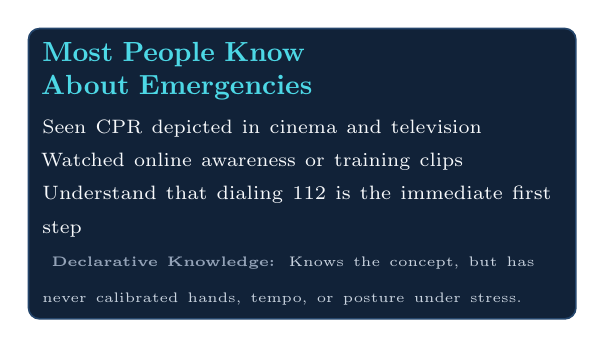
\begin{tikzpicture}
    \node[surface,text width=6.6cm,minimum height=1.95cm] {
      {\textbf{\teal{Most People Know}}\\\textbf{\teal{About Emergencies}}}\vspace{2pt}\newline
      \scriptsize
      $\blacktriangleright$ Seen CPR depicted in cinema and television\newline
      $\blacktriangleright$ Watched online awareness or training clips\newline
      $\blacktriangleright$ Understand that dialing 112 is the immediate first step\newline
      \vspace{1pt}
      \textcolor{TextMuted}{\tiny\textbf{Declarative Knowledge:}}
      \textcolor{TextSub}{\tiny Knows the concept, but has never calibrated hands, tempo, or posture under stress.}
    };
  \end{tikzpicture}

\column{0.49\textwidth}
  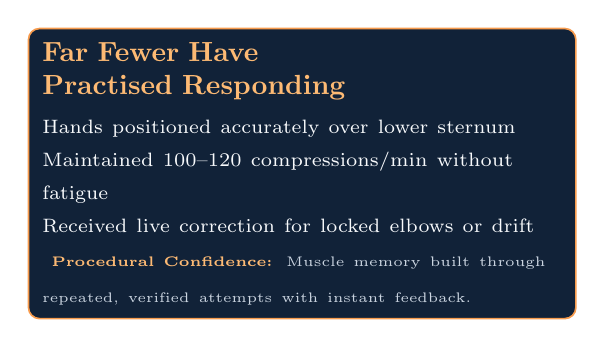
\begin{tikzpicture}
    \node[orangesurface,text width=6.6cm,minimum height=1.95cm] {
      {\textbf{\orange{Far Fewer Have}}\\\textbf{\orange{Practised Responding}}}\vspace{2pt}\newline
      \scriptsize
      $\blacktriangleright$ Hands positioned accurately over lower sternum\newline
      $\blacktriangleright$ Maintained 100--120 compressions/min without fatigue\newline
      $\blacktriangleright$ Received live correction for locked elbows or drift\newline
      \vspace{1pt}
      \textcolor{OrangeLight}{\tiny\textbf{Procedural Confidence:}}
      \textcolor{TextSub}{\tiny Muscle memory built through repeated, verified attempts with instant feedback.}
    };
  \end{tikzpicture}
\end{columns}

\vspace{0.00cm}

\begin{tikzpicture}
  \node[subtlebox,text width=14.1cm,inner sep=3pt,align=center] {
    \centering\textbf{\textcolor{TealLight}{\small``The problem is not lack of awareness. It is the absence of accessible, repeatable practice.''}}
  };
\end{tikzpicture}

\note{Open with a genuine, reflective question rather than a cold statistic. Give the audience a moment to reflect.
The key contrast is between declarative knowledge (knowing the steps) and procedural confidence (having performed and corrected them).
Estimated time: 30 seconds. Transition: "That gap — between knowing and having practised — is exactly what Sanjeevani is designed to close."}
\end{frame}

% ── SLIDE 3: WHY THIS MATTERS IN INDIA ─────────────────────
\begin{frame}{The Access Chasm in India}
\framesubtitle{Four systemic friction points limiting hands-on emergency training}

\vspace{-0.15cm}
\begin{columns}[T]
\column{0.49\textwidth}
  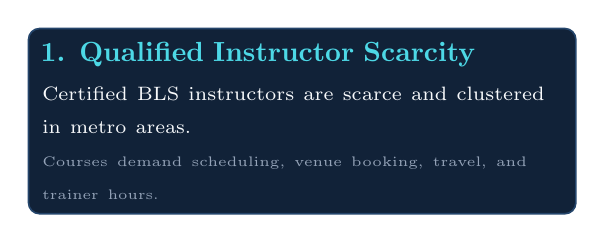
\begin{tikzpicture}
    \node[surface,text width=6.6cm,minimum height=1.95cm] {
      \textbf{\textcolor{TealLight}{1. Qualified Instructor Scarcity}}\vspace{2pt}\newline
      \scriptsize
      Certified BLS instructors are scarce and clustered in metro areas.\newline
      \textcolor{TextMuted}{\tiny Courses demand scheduling, venue booking, travel, and trainer hours.}
    };
  \end{tikzpicture}

  \vspace{0.06cm}

  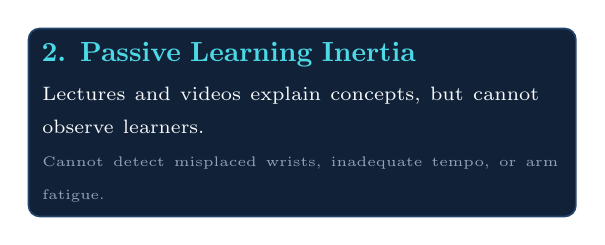
\begin{tikzpicture}
    \node[surface,text width=6.6cm,minimum height=1.95cm] {
      \textbf{\textcolor{TealLight}{2. Passive Learning Inertia}}\vspace{2pt}\newline
      \scriptsize
      Lectures and videos explain concepts, but cannot observe learners.\newline
      \textcolor{TextMuted}{\tiny Cannot detect misplaced wrists, inadequate tempo, or arm fatigue.}
    };
  \end{tikzpicture}

\column{0.49\textwidth}
  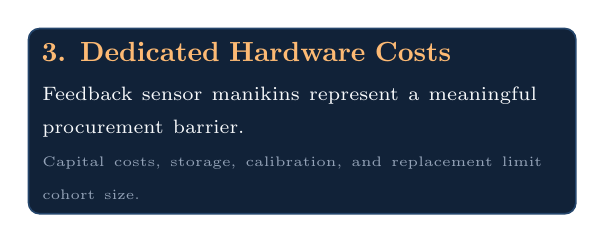
\begin{tikzpicture}
    \node[surface,text width=6.6cm,minimum height=1.95cm] {
      \textbf{\textcolor{OrangeLight}{3. Dedicated Hardware Costs}}\vspace{2pt}\newline
      \scriptsize
      Feedback sensor manikins represent a meaningful procurement barrier.\newline
      \textcolor{TextMuted}{\tiny Capital costs, storage, calibration, and replacement limit cohort size.}
    };
  \end{tikzpicture}

  \vspace{0.06cm}

  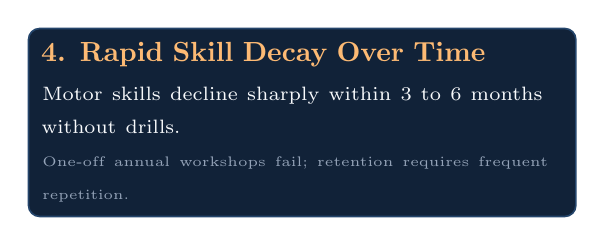
\begin{tikzpicture}
    \node[surface,text width=6.6cm,minimum height=1.95cm] {
      \textbf{\textcolor{OrangeLight}{4. Rapid Skill Decay Over Time}}\vspace{2pt}\newline
      \scriptsize
      Motor skills decline sharply within 3 to 6 months without drills.\newline
      \textcolor{TextMuted}{\tiny One-off annual workshops fail; retention requires frequent repetition.}
    };
  \end{tikzpicture}
\end{columns}

\vspace{0.08cm}

\begin{tikzpicture}
  \node[tealsurface,text width=14.1cm,inner sep=3.5pt,align=center] {
    \centering\textbf{\textcolor{TealLight}{\small``Information is already ubiquitous.\quad Scalable opportunities for interactive revision are not.''}}
  };
\end{tikzpicture}

\note{Present these as barriers to investigate — not universal deficits. Avoid claiming nobody in India has training.
The thesis: information is available. Opportunities to practise with feedback and correction are harder to come by consistently.
Time: ~50 seconds. Transition: "Let's look at why passive learning alone cannot solve this."}
\end{frame}

% ── SLIDE 4: WATCHING ≠ PRACTISING ────────────────────────
\begin{frame}{A Video Explains the Steps. Can It Correct Your Form?}
\framesubtitle{The biomechanical divide between passive observation and interactive correction}

\vspace{-0.15cm}
\begin{columns}[T]
\column{0.45\textwidth}
  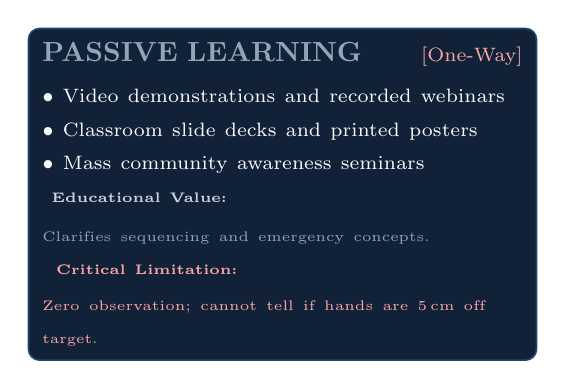
\begin{tikzpicture}
    \node[surface,text width=6.1cm,minimum height=3.5cm] {
      \textbf{\textcolor{TextMuted}{PASSIVE LEARNING}} \hfill \textcolor{RedLight}{\scriptsize[One-Way]}\vspace{3pt}\newline
      \scriptsize
      $\bullet$ Video demonstrations and recorded webinars\newline
      $\bullet$ Classroom slide decks and printed posters\newline
      $\bullet$ Mass community awareness seminars\newline
      \vspace{2pt}
      \textcolor{TextSub}{\tiny\textbf{Educational Value:}}\newline
      \textcolor{TextMuted}{\tiny Clarifies sequencing and emergency concepts.\newline}
      \vspace{1pt}
      \textcolor{RedLight}{\tiny\textbf{Critical Limitation:}}\newline
      \textcolor{RedLight}{\tiny Zero observation; cannot tell if hands are 5\,cm off target.}
    };
  \end{tikzpicture}

\column{0.08\textwidth}
  \begin{center}
    \vspace{1.5cm}
    
\begin{tikzpicture}
      \node[circle,fill=NavySurfaceLight,draw=TealLight,inner sep=3pt,text=TealLight,font=\scriptsize\bfseries] {VS};
      \draw[arrow,line width=1.3pt] (-0.3,-0.45) -- (0.3,-0.45);
    \end{tikzpicture}
  \end{center}

\column{0.45\textwidth}
  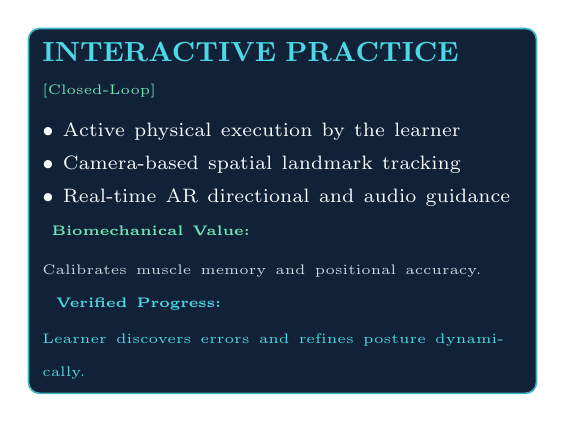
\begin{tikzpicture}
    \node[tealsurface,text width=6.1cm,minimum height=3.5cm] {
      \textbf{\textcolor{TealLight}{INTERACTIVE PRACTICE}} \hfill \textcolor{GreenLight}{\tiny[Closed-Loop]}\vspace{3pt}\newline
      \scriptsize
      $\bullet$ Active physical execution by the learner\newline
      $\bullet$ Camera-based spatial landmark tracking\newline
      $\bullet$ Real-time AR directional and audio guidance\newline
      \vspace{2pt}
      \textcolor{GreenLight}{\tiny\textbf{Biomechanical Value:}}\newline
      \textcolor{TextSub}{\tiny Calibrates muscle memory and positional accuracy.\newline}
      \vspace{1pt}
      \textcolor{TealLight}{\tiny\textbf{Verified Progress:}}\newline
      \textcolor{TealLight}{\tiny Learner discovers errors and refines posture dynamically.}
    };
  \end{tikzpicture}
\end{columns}

\vspace{0.08cm}

\begin{tikzpicture}
  \node[subtlebox,text width=14.1cm,inner sep=3.5pt,align=center] {
    \centering\textbf{\textcolor{TextMain}{\small``Watching teaches what the steps are.\quad Practising reveals what you can actually execute.''}}
  };
\end{tikzpicture}

\note{Make clear that videos and classroom teaching are valuable and should not be dismissed.
The argument is about the additional dimension of individual, repeated, corrective practice — not that passive learning is worthless.
Time: ~40 seconds. Transition: "The tool that most reliably provides that correction has historically been physical mannequins and instructors. Let's look at the economics of that."}
\end{frame}

% ── SLIDE 5: EQUIPMENT ECONOMICS ──────────────────────────
\begin{frame}{Physical Equipment is Vital --- But Hard to Scale for Revision}
\framesubtitle{Evaluating manikin tiers and the logistics of continuous institutional practice}

\vspace{-0.15cm}
\begin{columns}[T]
\column{0.53\textwidth}
  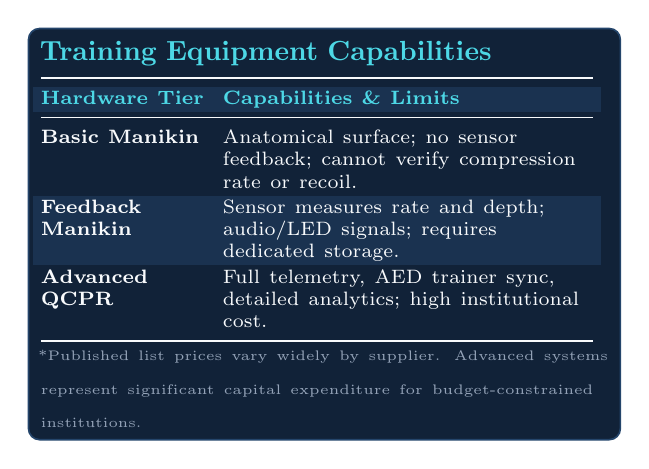
\begin{tikzpicture}
    \node[surface,text width=7.2cm,inner sep=4.5pt] {
      \textbf{\textcolor{TealLight}{Training Equipment Capabilities}}\vspace{3pt}\newline
      \scriptsize
      \setlength{\tabcolsep}{3pt}
      \renewcommand{\arraystretch}{1.15}
      \begin{tabular}{@{}>{\raggedright\arraybackslash}p{2.1cm}>{\raggedright\arraybackslash}p{4.7cm}@{}}
        \toprule
        \rowcolor{NavySurfaceLight}
        \textcolor{TealLight}{\textbf{Hardware Tier}} & \textcolor{TealLight}{\textbf{Capabilities \& Limits}} \\
        \midrule
        \rowcolor{NavySurface}
        \textbf{Basic Manikin} & Anatomical surface; no sensor feedback; cannot verify compression rate or recoil. \\
        \rowcolor{NavySurfaceLight}
        \textbf{Feedback Manikin} & Sensor measures rate and depth; audio/LED signals; requires dedicated storage. \\
        \rowcolor{NavySurface}
        \textbf{Advanced QCPR} & Full telemetry, AED trainer sync, detailed analytics; high institutional cost. \\
        \bottomrule
      \end{tabular}
      \vspace{2pt}\newline
      \textcolor{TextMuted}{\tiny *Published list prices vary widely by supplier. Advanced systems represent significant capital expenditure for budget-constrained institutions.}
    };
  \end{tikzpicture}

\column{0.45\textwidth}
  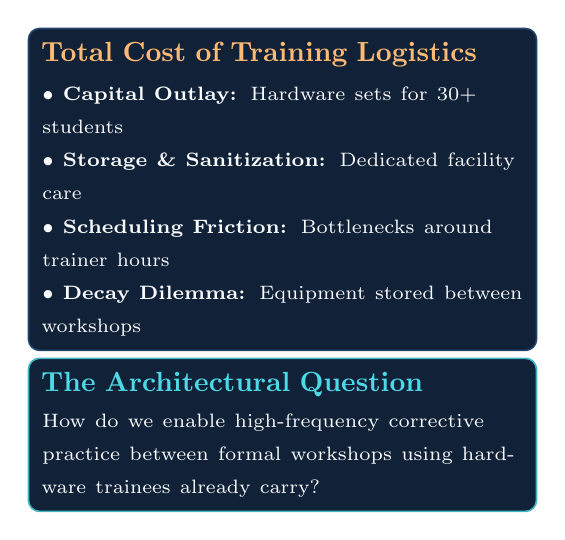
\begin{tikzpicture}
    \node[surface,text width=6.1cm] (costs) {
      \textbf{\textcolor{OrangeLight}{Total Cost of Training Logistics}}\vspace{2pt}\newline
      \scriptsize
      $\bullet$ \textbf{Capital Outlay:} Hardware sets for 30+ students\newline
      $\bullet$ \textbf{Storage \& Sanitization:} Dedicated facility care\newline
      $\bullet$ \textbf{Scheduling Friction:} Bottlenecks around trainer hours\newline
      $\bullet$ \textbf{Decay Dilemma:} Equipment stored between workshops
    };

    \node[tealsurface,text width=6.1cm,below=0.08cm of costs] {
      \textbf{\textcolor{TealLight}{The Architectural Question}}\vspace{1pt}\newline
      \scriptsize
      How do we enable high-frequency corrective practice between formal workshops using hardware trainees already carry?
    };
  \end{tikzpicture}
\end{columns}

\note{Do not state a single price range as universal. Basic manikins can cost a few thousand rupees; advanced feedback-enabled systems cost significantly more.
The point is about repeat access and revision frequency — not whether mannequins exist.
Time: ~45 seconds. Transition: "Before we show the solution, let's look at what established training programmes do well."}
\end{frame}

% ── SLIDE 6: WHAT ESTABLISHED TRAINING TEACHES US ─────────
\begin{frame}{Hands-On Emergency Training is an Established Global Model}
\framesubtitle{Learning from AHA and ERC standards while designing for Indian scale}

\vspace{-0.15cm}
\begin{columns}[T]
\column{0.49\textwidth}
  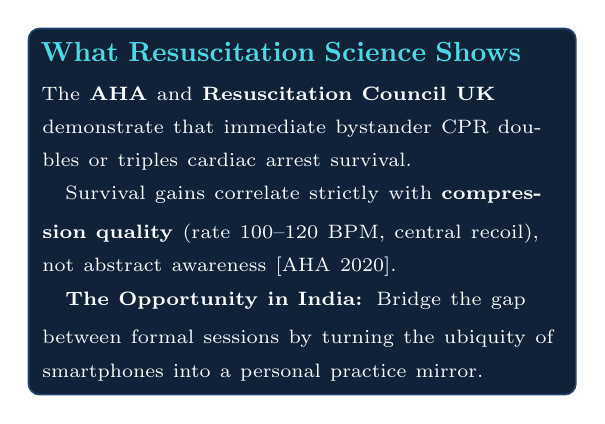
\begin{tikzpicture}
    \node[surface,text width=6.6cm,minimum height=3.6cm] {
      \textbf{\textcolor{TealLight}{What Resuscitation Science Shows}}\vspace{2pt}\newline
      \scriptsize
      $\blacktriangleright$ The \textbf{AHA} and \textbf{Resuscitation Council UK} demonstrate that immediate bystander CPR doubles or triples cardiac arrest survival.\newline
      \vspace{2pt}
      $\blacktriangleright$ Survival gains correlate strictly with \textbf{compression quality} (rate 100--120 BPM, central recoil), not abstract awareness [AHA 2020].\newline
      \vspace{2pt}
      $\blacktriangleright$ \textbf{The Opportunity in India:} Bridge the gap between formal sessions by turning the ubiquity of smartphones into a personal practice mirror.
    };
  \end{tikzpicture}

\column{0.49\textwidth}
  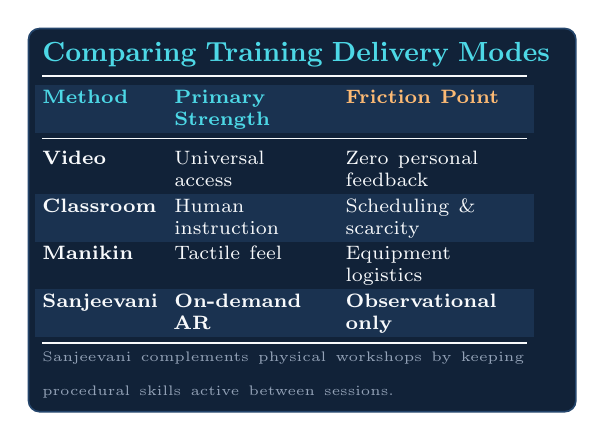
\begin{tikzpicture}
    \node[surface,text width=6.6cm,minimum height=3.6cm] {
      \textbf{\textcolor{TealLight}{Comparing Training Delivery Modes}}\vspace{2pt}\newline
      \scriptsize
      \setlength{\tabcolsep}{2.5pt}
      \renewcommand{\arraystretch}{1.15}
      \begin{tabular}{@{}>{\raggedright\arraybackslash}p{1.5cm}>{\raggedright\arraybackslash}p{2.0cm}>{\raggedright\arraybackslash}p{2.3cm}@{}}
        \toprule
        \rowcolor{NavySurfaceLight}
        \textcolor{TealLight}{\textbf{Method}} & \textcolor{TealLight}{\textbf{Primary Strength}} & \textcolor{OrangeLight}{\textbf{Friction Point}} \\
        \midrule
        \rowcolor{NavySurface}
        \textbf{Video} & Universal access & Zero personal feedback \\
        \rowcolor{NavySurfaceLight}
        \textbf{Classroom} & Human instruction & Scheduling \& scarcity \\
        \rowcolor{NavySurface}
        \textbf{Manikin} & Tactile feel & Equipment logistics \\
        \rowcolor{NavySurfaceLight}
        \textbf{Sanjeevani} & \textbf{On-demand AR} & \textbf{Observational only} \\
        \bottomrule
      \end{tabular}
      \vspace{2pt}\newline
      \textcolor{TextMuted}{\tiny Sanjeevani complements physical workshops by keeping procedural skills active between sessions.}
    };
  \end{tikzpicture}
\end{columns}

\vspace{0.08cm}

\begin{tikzpicture}
  \node[subtlebox,text width=14.1cm,inner sep=3.5pt,align=center] {
    \centering\footnotesize\textcolor{TextSub}{``Sanjeevani adopts the hands-on feedback philosophy of AHA/ERC and delivers it via on-device mobile vision.''}
  };
\end{tikzpicture}

\note{Cite AHA and Red Cross accurately — they recommend hands-on practice, not just classroom instruction.
Do NOT claim all Western citizens receive training or that India has no trained instructors.
The goal is to show that Sanjeevani aligns with what established programmes value (hands-on repetition) while adapting delivery to local constraints.
Time: ~50 seconds. Transition: "So — what is Sanjeevani, and how does it aim to close this gap?"}
\end{frame}

% ── SLIDE 7: INTRODUCING SANJEEVANI ───────────────────────
\begin{frame}{Practice That Starts With the Phone in Your Pocket}
\framesubtitle{Introducing Sanjeevani --- An on-device Android emergency-skills training platform}

\vspace{-0.27cm}
\begin{columns}[T]
\column{0.57\textwidth}
  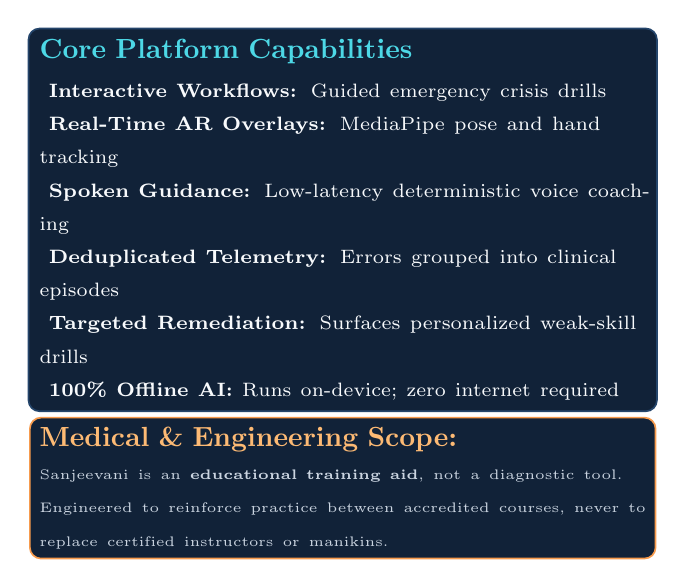
\begin{tikzpicture}
    \node[surface,text width=7.7cm,inner sep=4pt] (feat) {
      \textbf{\textcolor{TealLight}{Core Platform Capabilities}}\vspace{2pt}\newline
      \scriptsize
      \textcolor{GreenLight}{\textbf{$\checkmark$}} \textbf{Interactive Workflows:} Guided emergency crisis drills\newline
      \textcolor{GreenLight}{\textbf{$\checkmark$}} \textbf{Real-Time AR Overlays:} MediaPipe pose and hand tracking\newline
      \textcolor{GreenLight}{\textbf{$\checkmark$}} \textbf{Spoken Guidance:} Low-latency deterministic voice coaching\newline
      \textcolor{GreenLight}{\textbf{$\checkmark$}} \textbf{Deduplicated Telemetry:} Errors grouped into clinical episodes\newline
      \textcolor{GreenLight}{\textbf{$\checkmark$}} \textbf{Targeted Remediation:} Surfaces personalized weak-skill drills\newline
      \textcolor{GreenLight}{\textbf{$\checkmark$}} \textbf{100\% Offline AI:} Runs on-device; zero internet required
    };

    \node[orangesurface,text width=7.7cm,inner sep=3.5pt,below=0.06cm of feat] {
      \textbf{\textcolor{OrangeLight}{Medical \& Engineering Scope:}}\newline
      \tiny\textcolor{TextSub}{Sanjeevani is an \textbf{educational training aid}, not a diagnostic tool. Engineered to reinforce practice between accredited courses, never to replace certified instructors or manikins.}
    };
  \end{tikzpicture}

\column{0.41\textwidth}
  \begin{center}
    % Sleek vector phone mockup
    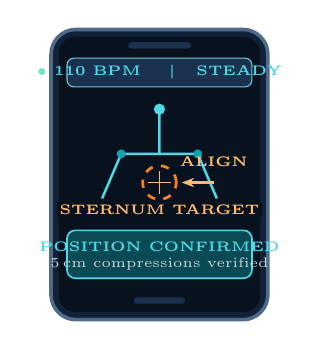
\begin{tikzpicture}[scale=0.81]
      % phone bezel
      \draw[NavyBorder!80,fill=NavySurface,rounded corners=9pt,line width=1.3pt]
            (0,0) rectangle (3.4,4.55);
      % screen area
      \fill[NavyBg,rounded corners=6pt] (0.12,0.12) rectangle (3.28,4.43);
      % top speaker notch
      \fill[NavySurfaceLight,rounded corners=1.5pt] (1.2,4.25) rectangle (2.2,4.35);

      % Metronome HUD widget (inside screen)
      \fill[NavySurfaceLight,rounded corners=2.5pt,draw=Teal!60]
            (0.25,3.65) rectangle (3.15,4.1);
      \node[text=TealLight,font=\tiny\bfseries,align=center] at (1.7,3.88)
           {\textcolor{GreenLight}{$\bullet$}\ 110 BPM \quad\textbar\quad STEADY};

      % AR skeleton lines
      \draw[TealLight,line width=0.9pt]
            (1.1,2.6) -- (2.3,2.6)
            (1.7,2.6) -- (1.7,3.3)
            (1.1,2.6) -- (0.8,1.9)
            (2.3,2.6) -- (2.6,1.9);
      \fill[TealLight] (1.7,3.3) circle (2.5pt); % head
      \fill[Teal] (1.1,2.6) circle (2pt);       % left shoulder
      \fill[Teal] (2.3,2.6) circle (2pt);       % right shoulder

      % Sternum target with crosshair
      \draw[Orange,dashed,line width=1.0pt] (1.7,2.15) circle (7.5pt);
      \draw[OrangeLight,line width=0.5pt] (1.52,2.15) -- (1.88,2.15);
      \draw[OrangeLight,line width=0.5pt] (1.7,1.97) -- (1.7,2.33);

      % Correction vector arrow & label
      \draw[arrowO,line width=1.3pt] (2.55,2.15) -- (2.05,2.15);
      \node[OrangeLight,font=\fontsize{4.5pt}{5.5pt}\selectfont\bfseries,fill=NavyBg,inner sep=1pt,rounded corners=1pt] at (1.7,1.72) {STERNUM TARGET};
      \node[OrangeLight,font=\fontsize{4.5pt}{5.5pt}\selectfont\bfseries,anchor=south] at (2.55,2.25) {ALIGN};

      % Live guidance card (inside screen)
      \fill[TealDark,rounded corners=3pt,draw=TealLight,line width=0.6pt]
            (0.25,0.65) rectangle (3.15,1.40);
      \node[text=TealLight,font=\fontsize{5pt}{6pt}\selectfont\bfseries] at (1.7,1.15) {POSITION CONFIRMED};
      \node[text=TextSub,font=\fontsize{4pt}{5pt}\selectfont] at (1.7,0.88) {5\,cm compressions verified};

      % Bottom navigation indicator
      \fill[NavySurfaceLight,rounded corners=1pt] (1.3,0.25) rectangle (2.1,0.35);
    \end{tikzpicture}
  \end{center}
\end{columns}

\note{Introduce Sanjeevani clearly as a training tool, not a substitute for emergency services or qualified instruction.
Key phrase: "the phone you already have" emphasises accessibility without hardware investment.
Time: ~45 seconds. Transition: "Let me show you the core learning loop that powers all modules."}
\end{frame}

% ── SLIDE 8: THE LEARNING LOOP ─────────────────────────────
\begin{frame}{The 7-Stage Closed Learning Loop}
\framesubtitle{Continuous cycle: instruction, sensor observation, correction, and telemetry}

\vspace{-0.15cm}
\begin{center}
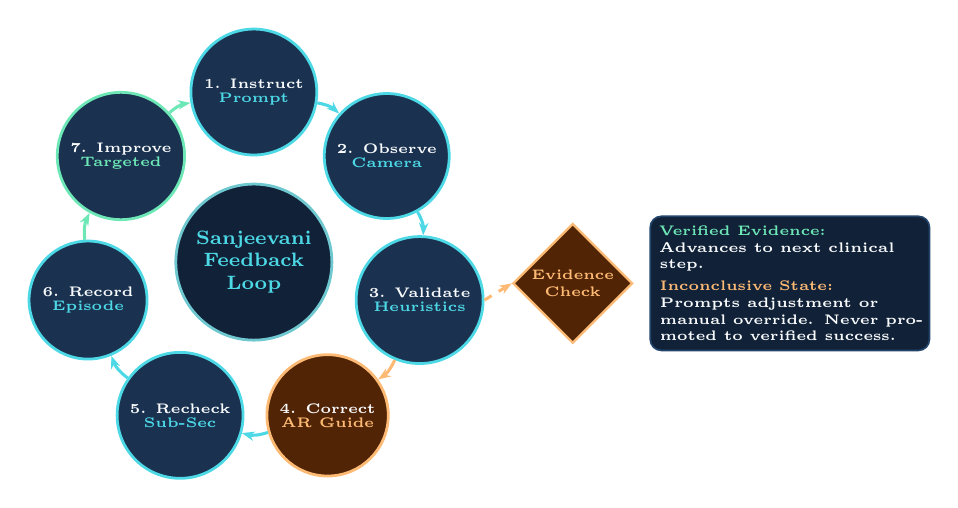
\begin{tikzpicture}[every node/.style={font=\tiny\bfseries},scale=0.90]
  % 7 nodes on circle of radius 2.4cm
  \node[circle,fill=NavySurfaceLight,draw=TealLight,line width=1pt,
        minimum size=1.1cm,text=TextMain,align=center]
       (n0) at (90:2.4)    {1. Instruct\\[-1pt]\tiny\textcolor{TealLight}{Prompt}};
  \node[circle,fill=NavySurfaceLight,draw=TealLight,line width=1pt,
        minimum size=1.1cm,text=TextMain,align=center]
       (n1) at (38.6:2.4)  {2. Observe\\[-1pt]\tiny\textcolor{TealLight}{Camera}};
  \node[circle,fill=NavySurfaceLight,draw=TealLight,line width=1pt,
        minimum size=1.1cm,text=TextMain,align=center]
       (n2) at (-12.9:2.4) {3. Validate\\[-1pt]\tiny\textcolor{TealLight}{Heuristics}};
  \node[circle,fill=OrangeDark,draw=OrangeLight,line width=1pt,
        minimum size=1.1cm,text=TextMain,align=center]
       (n3) at (-64.3:2.4) {4. Correct\\[-1pt]\tiny\textcolor{OrangeLight}{AR Guide}};
  \node[circle,fill=NavySurfaceLight,draw=TealLight,line width=1pt,
        minimum size=1.1cm,text=TextMain,align=center]
       (n4) at (-115.7:2.4){5. Recheck\\[-1pt]\tiny\textcolor{TealLight}{Sub-Sec}};
  \node[circle,fill=NavySurfaceLight,draw=TealLight,line width=1pt,
        minimum size=1.1cm,text=TextMain,align=center]
       (n5) at (-167.1:2.4){6. Record\\[-1pt]\tiny\textcolor{TealLight}{Episode}};
  \node[circle,fill=NavySurfaceLight,draw=GreenLight,line width=1pt,
        minimum size=1.1cm,text=TextMain,align=center]
       (n6) at (-218.6:2.4){7. Improve\\[-1pt]\tiny\textcolor{GreenLight}{Targeted}};

  % arrows around loop
  \draw[arrow] (n0) to[bend left=16] (n1);
  \draw[arrow] (n1) to[bend left=16] (n2);
  \draw[arrowO] (n2) to[bend left=16] (n3);
  \draw[arrow] (n3) to[bend left=16] (n4);
  \draw[arrow] (n4) to[bend left=16] (n5);
  \draw[arrowG] (n5) to[bend left=16] (n6);
  \draw[arrowG] (n6) to[bend left=16] (n0);

  % center badge
  \node[circle,fill=NavySurface,draw=Teal!60,line width=1pt,minimum size=1.3cm,
        text=TealLight,font=\scriptsize\bfseries,align=center] at (0,0)
       {Sanjeevani\\Feedback\\Loop};

  % Honest Engineering Diamond off Validate
  \node[shape=diamond,fill=OrangeDark,draw=OrangeLight,line width=0.8pt,font=\tiny\bfseries,
        minimum size=0.95cm,align=center,inner sep=1pt,text=OrangeLight]
       (dec) at (4.5,-0.3) {Evidence\\Check};

  \draw[arrowO,dashed] (n2.east) -- (dec.west);

  \node[surface,draw=NavyBorder,text width=3.3cm,right=0.2cm of dec,inner sep=3.5pt] {
    \textcolor{GreenLight}{\textbf{Verified Evidence:}}\newline
    \tiny Advances to next clinical step.\\[2pt]
    \textcolor{OrangeLight}{\textbf{Inconclusive State:}}\newline
    \tiny Prompts adjustment or manual override. Never promoted to verified success.
  };
\end{tikzpicture}
\end{center}

\vspace{-0.15cm}

\begin{tikzpicture}
  \node[subtlebox,text width=14.1cm,inner sep=3.5pt,align=center] {
    \centering\footnotesize\textcolor{TextSub}{The decision diamond represents honest engineering: when camera tracking is uncertain, the system declares an inconclusive state rather than reporting false mastery.}
  };
\end{tikzpicture}

\note{Walk through each node in ~5 seconds each. Emphasise the "Validate" step — this is where honest engineering lives.
When there is not enough evidence, the app shows uncertainty and offers retry or tap-to-continue.
Manual continuation is never silently treated as verified success.
Time: ~55 seconds. Transition: "That loop powers our emergency modules."}
\end{frame}

% ── SLIDE 9: THE FOUR MODULES ─────────────────────────────
\begin{frame}{One Engine. Four Critical Emergency Scenarios.}
\framesubtitle{Unified computer vision architecture tailored for distinct medical protocols}

\vspace{-0.24cm}
\begin{columns}[T]
\column{0.245\textwidth}
  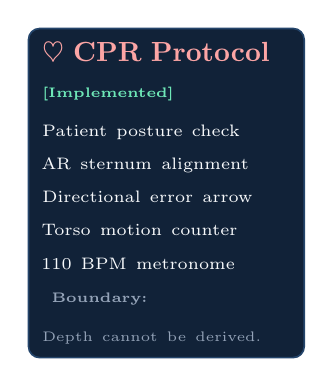
\begin{tikzpicture}
    \node[surface,text width=3.15cm,minimum height=3.35cm] {
      \textbf{\textcolor{RedLight}{$\heartsuit$ CPR Protocol}}\vspace{1pt}\newline
      \tiny\textcolor{GreenLight}{\textbf{[Implemented]}}\vspace{2pt}\newline
      \fontsize{6.5pt}{7.8pt}\selectfont
      $\checkmark$ Patient posture check\newline
      $\checkmark$ AR sternum alignment\newline
      $\checkmark$ Directional error arrow\newline
      $\checkmark$ Torso motion counter\newline
      $\checkmark$ 110 BPM metronome\newline
      \vspace{2pt}
      \textcolor{TextMuted}{\tiny\textbf{Boundary:}}\newline
      \textcolor{TextMuted}{\tiny Depth cannot be derived.}
    };
  \end{tikzpicture}

\column{0.245\textwidth}
  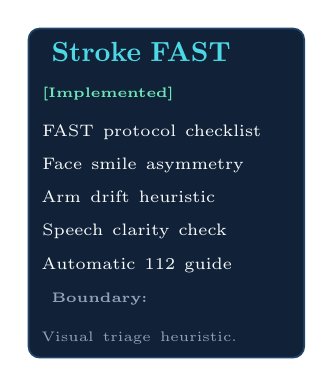
\begin{tikzpicture}
    \node[surface,text width=3.15cm,minimum height=3.35cm] {
      \textbf{\textcolor{TealLight}{$\bigstar$ Stroke FAST}}\vspace{1pt}\newline
      \tiny\textcolor{GreenLight}{\textbf{[Implemented]}}\vspace{2pt}\newline
      \fontsize{6.5pt}{7.8pt}\selectfont
      $\checkmark$ FAST protocol checklist\newline
      $\checkmark$ Face smile asymmetry\newline
      $\checkmark$ Arm drift heuristic\newline
      $\checkmark$ Speech clarity check\newline
      $\checkmark$ Automatic 112 guide\newline
      \vspace{2pt}
      \textcolor{TextMuted}{\tiny\textbf{Boundary:}}\newline
      \textcolor{TextMuted}{\tiny Visual triage heuristic.}
    };
  \end{tikzpicture}

\column{0.245\textwidth}
  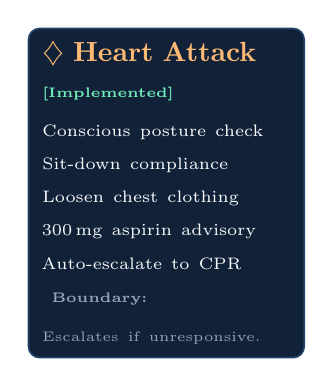
\begin{tikzpicture}
    \node[surface,text width=3.15cm,minimum height=3.35cm] {
      \textbf{\textcolor{OrangeLight}{$\diamondsuit$ Heart Attack}}\vspace{1pt}\newline
      \tiny\textcolor{GreenLight}{\textbf{[Implemented]}}\vspace{2pt}\newline
      \fontsize{6.5pt}{7.8pt}\selectfont
      $\checkmark$ Conscious posture check\newline
      $\checkmark$ Sit-down compliance\newline
      $\checkmark$ Loosen chest clothing\newline
      $\checkmark$ 300\,mg aspirin advisory\newline
      $\checkmark$ Auto-escalate to CPR\newline
      \vspace{2pt}
      \textcolor{TextMuted}{\tiny\textbf{Boundary:}}\newline
      \textcolor{TextMuted}{\tiny Escalates if unresponsive.}
    };
  \end{tikzpicture}

\column{0.245\textwidth}
  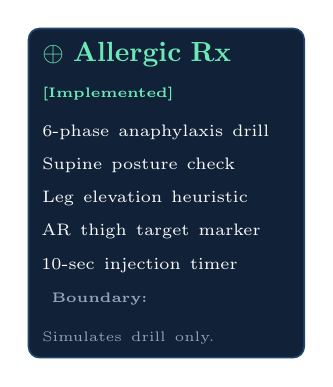
\begin{tikzpicture}
    \node[surface,text width=3.15cm,minimum height=3.35cm] {
      \textbf{\textcolor{GreenLight}{$\oplus$ Allergic Rx}}\vspace{1pt}\newline
      \tiny\textcolor{GreenLight}{\textbf{[Implemented]}}\vspace{2pt}\newline
      \fontsize{6.5pt}{7.8pt}\selectfont
      $\checkmark$ 6-phase anaphylaxis drill\newline
      $\checkmark$ Supine posture check\newline
      $\checkmark$ Leg elevation heuristic\newline
      $\checkmark$ AR thigh target marker\newline
      $\checkmark$ 10-sec injection timer\newline
      \vspace{2pt}
      \textcolor{TextMuted}{\tiny\textbf{Boundary:}}\newline
      \textcolor{TextMuted}{\tiny Simulates drill only.}
    };
  \end{tikzpicture}
\end{columns}

\vspace{0.05cm}

\begin{tikzpicture}
  \node[subtlebox,text width=14.1cm,inner sep=3pt,align=center] {
    \centering\scriptsize\textcolor{TextSub}{Choking and Recovery Position protocols listed in roadmap. All medical training content subject to qualified clinical review.}
  };
\end{tikzpicture}

\note{Be explicit that each module uses camera differently — not all four are identical.
Stroke and Allergy camera assessments are heuristic observations, not clinical measurements.
Time: ~55 seconds. Transition: "Let me show you the product working."}
\end{frame}

% ── SLIDE 10: LIVE DEMONSTRATION ───────────────────────────
\begin{frame}{See the Learning Loop in Action}
\framesubtitle{Live demonstration on an Android smartphone}

\vspace{-0.15cm}
\begin{columns}[T]
\column{0.57\textwidth}
  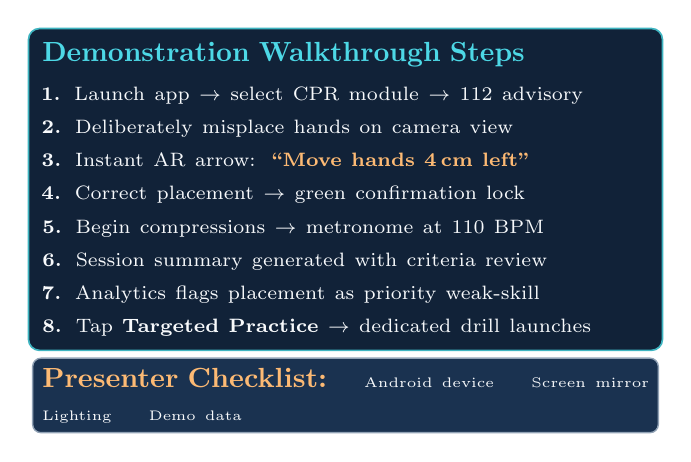
\begin{tikzpicture}
    \node[tealsurface,text width=7.7cm] (seq) {
      \textbf{\textcolor{TealLight}{Demonstration Walkthrough Steps}}\vspace{2pt}\newline
      \scriptsize
      \textbf{1.} Launch app $\rightarrow$ select CPR module $\rightarrow$ 112 advisory\newline
      \textbf{2.} Deliberately misplace hands on camera view\newline
      \textbf{3.} Instant AR arrow: \textcolor{OrangeLight}{\textbf{``Move hands 4\,cm left''}}\newline
      \textbf{4.} Correct placement $\rightarrow$ green confirmation lock\newline
      \textbf{5.} Begin compressions $\rightarrow$ metronome at 110 BPM\newline
      \textbf{6.} Session summary generated with criteria review\newline
      \textbf{7.} Analytics flags placement as priority weak-skill\newline
      \textbf{8.} Tap \textbf{Targeted Practice} $\rightarrow$ dedicated drill launches
    };

    \node[subtlebox,text width=7.7cm,below=0.08cm of seq] {
      \textbf{\textcolor{OrangeLight}{Presenter Checklist:}}\quad
      \tiny$\square$\ Android device \quad $\square$\ Screen mirror \quad $\square$\ Lighting \quad $\square$\ Demo data
    };
  \end{tikzpicture}

\column{0.41\textwidth}
  \begin{center}
    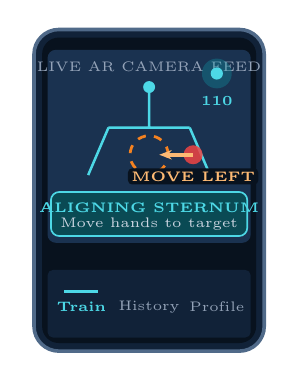
\begin{tikzpicture}[scale=0.86]
      % Phone bezel
      \draw[NavyBorder!80,fill=NavySurface,rounded corners=9pt,line width=1.3pt]
            (0,0) rectangle (3.4,4.75);
      \fill[NavyBg,rounded corners=6pt] (0.12,0.12) rectangle (3.28,4.63);

      % Camera preview backdrop
      \fill[NavySurfaceLight,rounded corners=3pt] (0.2,1.6) rectangle (3.2,4.45);
      \node[text=TextMuted,font=\tiny] at (1.7,4.2) {LIVE AR CAMERA FEED};

      % Metronome sphere
      \fill[Teal,opacity=0.3] (2.7,4.1) circle (0.22cm);
      \fill[TealLight] (2.7,4.1) circle (0.09cm);
      \node[text=TealLight,font=\tiny\bfseries,anchor=north] at (2.7,3.9) {110};

      % Pose skeleton
      \draw[TealLight,line width=0.9pt]
            (1.1,3.3) -- (2.3,3.3)
            (1.7,3.3) -- (1.7,3.9)
            (1.1,3.3) -- (0.8,2.6)
            (2.3,3.3) -- (2.6,2.6);
      \fill[TealLight] (1.7,3.9) circle (2.5pt);

      % Sternum target
      \draw[Orange,dashed,line width=1.0pt] (1.7,2.9) circle (8pt);

      % Misplaced hand indicator + correction vector
      \fill[Red,opacity=0.85] (2.35,2.9) circle (4pt);
      \draw[arrowO,line width=1.4pt] (2.35,2.9) -- (1.85,2.9);
      \node[OrangeLight,font=\fontsize{4.5pt}{5.5pt}\selectfont\bfseries,fill=NavyBg,inner sep=1.2pt,rounded corners=1.5pt] at (2.35,2.58) {MOVE LEFT};

      % Dynamic HUD pill (inside bezel)
      \fill[TealDark,rounded corners=3pt,draw=TealLight,line width=0.6pt] (0.25,1.7) rectangle (3.15,2.35);
      \node[text=TealLight,font=\tiny\bfseries] at (1.7,2.12) {ALIGNING STERNUM};
      \node[text=TextSub,font=\fontsize{4pt}{5pt}\selectfont] at (1.7,1.88) {Move hands to target};

      % Bottom navigation tabs
      \fill[NavySurface,rounded corners=2pt] (0.2,0.2) rectangle (3.2,1.2);
      \node[text=TealLight,font=\fontsize{5.5pt}{6.5pt}\selectfont\bfseries] at (0.7,0.65) {Train};
      \node[text=TextMuted,font=\fontsize{5pt}{6pt}\selectfont] at (1.7,0.65) {History};
      \node[text=TextMuted,font=\fontsize{5pt}{6pt}\selectfont] at (2.7,0.65) {Profile};
      \draw[TealLight,line width=1.3pt] (0.45,0.88) -- (0.95,0.88);
    \end{tikzpicture}
  \end{center}
\end{columns}

\note{Do NOT simulate successful tracking — show the actual app.
If the camera does not detect the target, that is honest: show the INCONCLUSIVE state and explain the fallback.
The key demonstration moments: (1) correction arrow, (2) position confirmed, (3) BPM metronome in HUD, (4) session report to targeted practice.
Time: ~90 seconds. Transition: "What you saw there is built on our analytics layer."}
\end{frame}

% ── SLIDE 11: ERRORS → PERSONALIZED PRACTICE ──────────────
\begin{frame}{From Observed Errors to Targeted Practice}
\framesubtitle{Connecting computer vision telemetry to personalized skill remediation}

\vspace{0.02cm}
\begin{center}
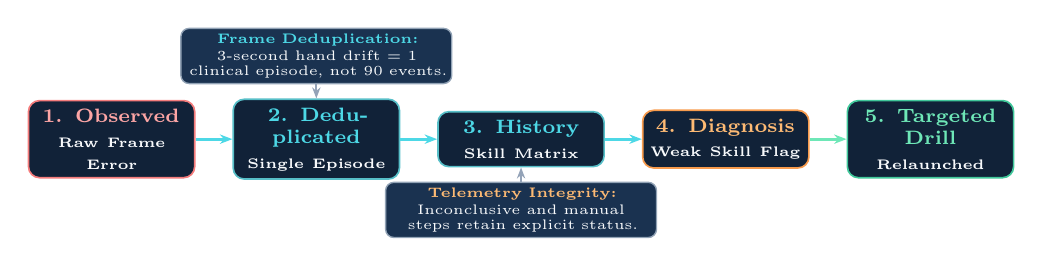
\begin{tikzpicture}[every node/.style={font=\scriptsize\bfseries}]
  \node[surface,draw=Red!70,minimum width=2.1cm,text width=1.9cm,align=center,inner sep=3pt] (obs) at (-5.2,0)
       {\textcolor{RedLight}{1. Observed}\\[1pt]\tiny Raw Frame Error};

  \node[surface,draw=Teal!70,minimum width=2.1cm,text width=1.9cm,align=center,inner sep=3pt] (ep) at (-2.6,0)
       {\textcolor{TealLight}{2. Deduplicated}\\[1pt]\tiny Single Episode};

  \node[surface,draw=Teal!70,minimum width=2.1cm,text width=1.9cm,align=center,inner sep=3pt] (hist) at (0.0,0)
       {\textcolor{TealLight}{3. History}\\[1pt]\tiny Skill Matrix};

  \node[orangesurface,minimum width=2.1cm,text width=1.9cm,align=center,inner sep=3pt] (diag) at (2.6,0)
       {\textcolor{OrangeLight}{4. Diagnosis}\\[1pt]\tiny Weak Skill Flag};

  \node[greensurface,minimum width=2.1cm,text width=1.9cm,align=center,inner sep=3pt] (drill) at (5.2,0)
       {\textcolor{GreenLight}{5. Targeted Drill}\\[1pt]\tiny Relaunched};

  \draw[arrow] (obs) -- (ep);
  \draw[arrow] (ep) -- (hist);
  \draw[arrow] (hist) -- (diag);
  \draw[arrowG] (diag) -- (drill);

  % Top callout on Deduplication
  \node[subtlebox,font=\fontsize{4.5pt}{5.5pt}\selectfont,above=0.18cm of ep,text width=3.3cm,align=center,inner sep=2pt] (dedup)
       {\textcolor{TealLight}{\textbf{Frame Deduplication:}}\\[0.5pt]
        3-second hand drift = 1 clinical episode, not 90 events.};
  \draw[arrowDashed] (dedup) -- (ep);

  % Bottom callout on Inconclusive integrity
  \node[subtlebox,font=\fontsize{4.5pt}{5.5pt}\selectfont,below=0.18cm of hist,text width=3.3cm,align=center,inner sep=2pt] (incon)
       {\textcolor{OrangeLight}{\textbf{Telemetry Integrity:}}\\[0.5pt]
        Inconclusive and manual steps retain explicit status.};
  \draw[arrowDashed] (incon) -- (hist);
\end{tikzpicture}
\end{center}

\vspace{-0.26cm}
\begin{columns}[T]
\column{0.49\textwidth}
  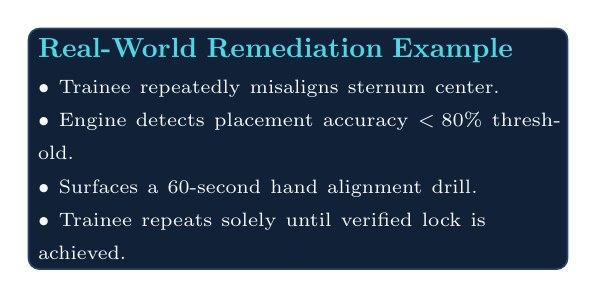
\begin{tikzpicture}
    \node[surface,text width=6.6cm,minimum height=1.75cm,inner sep=3.5pt] {
      \textbf{\textcolor{TealLight}{Real-World Remediation Example}}\vspace{1pt}\newline
      \scriptsize
      $\bullet$ Trainee repeatedly misaligns sternum center.\newline
      $\bullet$ Engine detects placement accuracy $<80\%$ threshold.\newline
      $\bullet$ Surfaces a 60-second hand alignment drill.\newline
      $\bullet$ Trainee repeats solely until verified lock is achieved.
    };
  \end{tikzpicture}

\column{0.49\textwidth}
  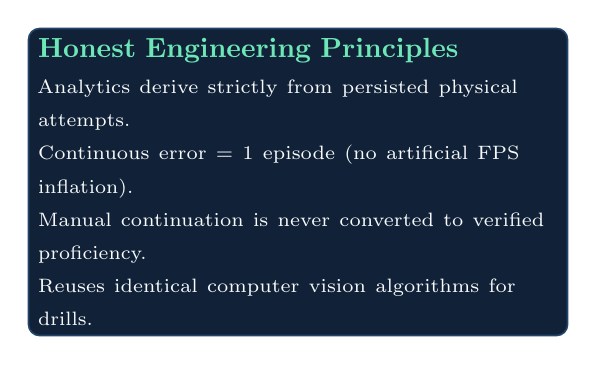
\begin{tikzpicture}
    \node[surface,text width=6.6cm,minimum height=1.75cm,inner sep=3.5pt] {
      \textbf{\textcolor{GreenLight}{Honest Engineering Principles}}\vspace{1pt}\newline
      \scriptsize
      $\checkmark$ Analytics derive strictly from persisted physical attempts.\newline
      $\checkmark$ Continuous error = 1 episode (no artificial FPS inflation).\newline
      $\checkmark$ Manual continuation is never converted to verified proficiency.\newline
      $\checkmark$ Reuses identical computer vision algorithms for drills.
    };
  \end{tikzpicture}
\end{columns}

\note{The key engineering honesty point: we do not inflate error counts by counting each camera frame.
One continuous positioning error = one episode.
Analytics are meaningful because they come from real events, not synthetic counters.
Time: ~50 seconds. Transition: "Now — what does this all mean for affordability and deployment?"}
\end{frame}

% ── SLIDE 12: AFFORDABILITY ────────────────────────────────
\begin{frame}{Lowering the Barrier to Practice --- Not the Standard of Care}
\framesubtitle{How Sanjeevani fits into the institutional first-aid training ecosystem}

\vspace{-0.15cm}
\begin{columns}[T]
\column{0.50\textwidth}
  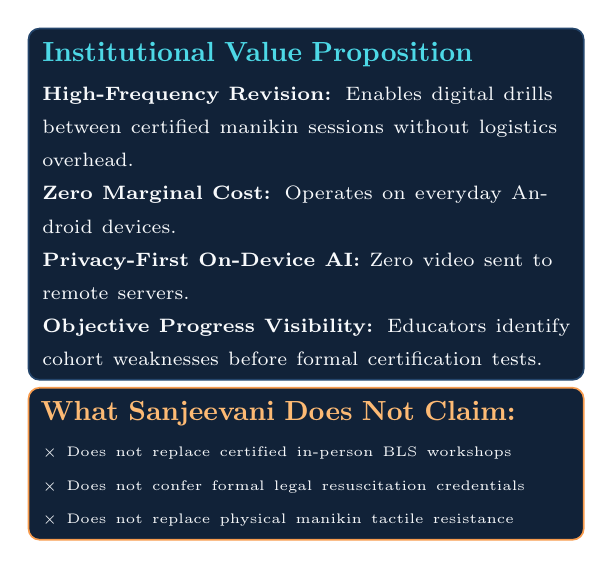
\begin{tikzpicture}
    \node[surface,text width=6.7cm] (ben) {
      \textbf{\textcolor{TealLight}{Institutional Value Proposition}}\vspace{2pt}\newline
      \scriptsize
      $\blacktriangleright$ \textbf{High-Frequency Revision:} Enables digital drills between certified manikin sessions without logistics overhead.\newline
      $\blacktriangleright$ \textbf{Zero Marginal Cost:} Operates on everyday Android devices.\newline
      $\blacktriangleright$ \textbf{Privacy-First On-Device AI:} Zero video sent to remote servers.\newline
      $\blacktriangleright$ \textbf{Objective Progress Visibility:} Educators identify cohort weaknesses before formal certification tests.
    };

    \node[orangesurface,text width=6.7cm,below=0.08cm of ben] {
      \textbf{\textcolor{OrangeLight}{What Sanjeevani Does Not Claim:}}\vspace{1pt}\newline
      \tiny
      $\times$ Does not replace certified in-person BLS workshops\newline
      $\times$ Does not confer formal legal resuscitation credentials\newline
      $\times$ Does not replace physical manikin tactile resistance
    };
  \end{tikzpicture}

\column{0.48\textwidth}
  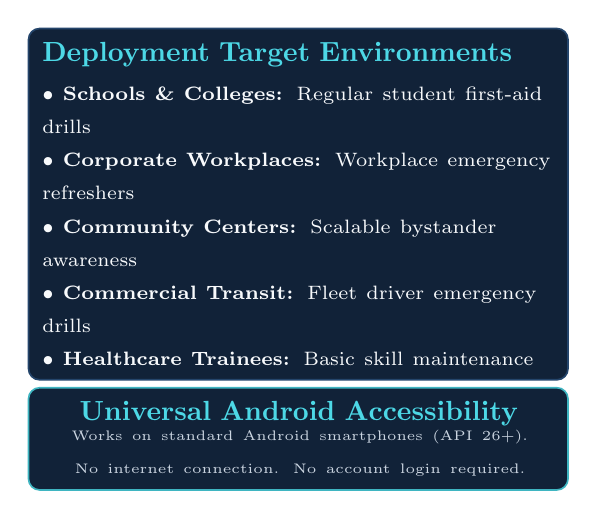
\begin{tikzpicture}
    \node[surface,text width=6.5cm] (dep) {
      \textbf{\textcolor{TealLight}{Deployment Target Environments}}\vspace{2pt}\newline
      \scriptsize
      $\bullet$ \textbf{Schools \& Colleges:} Regular student first-aid drills\newline
      $\bullet$ \textbf{Corporate Workplaces:} Workplace emergency refreshers\newline
      $\bullet$ \textbf{Community Centers:} Scalable bystander awareness\newline
      $\bullet$ \textbf{Commercial Transit:} Fleet driver emergency drills\newline
      $\bullet$ \textbf{Healthcare Trainees:} Basic skill maintenance
    };

    \node[tealsurface,text width=6.5cm,below=0.08cm of dep,align=center] {
      \centering\textbf{\textcolor{TealLight}{Universal Android Accessibility}}\\[1pt]
      \tiny\textcolor{TextSub}{Works on standard Android smartphones (API 26+).\\No internet connection. No account login required.}
    };
  \end{tikzpicture}
\end{columns}

\note{The accessibility argument is about repeat revision between sessions — not eliminating sessions.
Position Sanjeevani as a complement, not a replacement.
Do not claim cost savings without data from a real comparative study.
Time: ~45 seconds. Transition: "For Sanjeevani to be trusted, learning must be measurable."}
\end{frame}

% ── SLIDE 13: VALIDATION AND IMPACT ───────────────────────
\begin{frame}{Measuring Verified Competence --- Not Vanity Downloads}
\framesubtitle{Proposed evaluation metrics and pilot study framework}

\vspace{-0.22cm}
\begin{columns}[T]
\column{0.49\textwidth}
  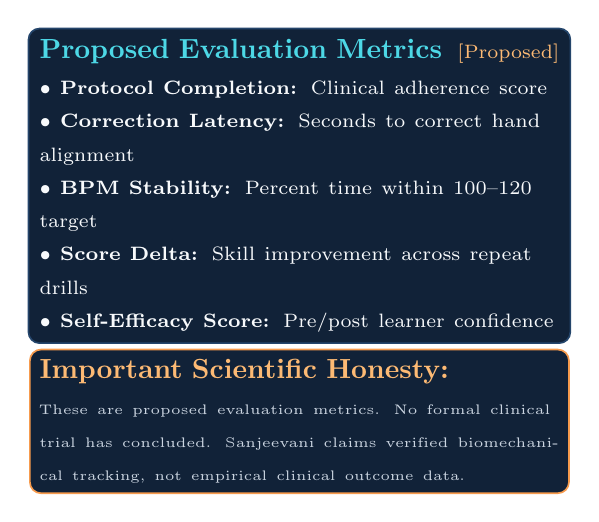
\begin{tikzpicture}
    \node[surface,text width=6.6cm,inner sep=4pt] (metrics) {
      \textbf{\textcolor{TealLight}{Proposed Evaluation Metrics}} \hfill \textcolor{OrangeLight}{\scriptsize[Proposed]}\vspace{1pt}\newline
      \scriptsize
      $\bullet$ \textbf{Protocol Completion:} Clinical adherence score\newline
      $\bullet$ \textbf{Correction Latency:} Seconds to correct hand alignment\newline
      $\bullet$ \textbf{BPM Stability:} Percent time within 100--120 target\newline
      $\bullet$ \textbf{Score Delta:} Skill improvement across repeat drills\newline
      $\bullet$ \textbf{Self-Efficacy Score:} Pre/post learner confidence
    };

    \node[orangesurface,text width=6.6cm,inner sep=3.5pt,below=0.06cm of metrics] {
      \textbf{\textcolor{OrangeLight}{Important Scientific Honesty:}}\vspace{1pt}\newline
      \tiny\textcolor{TextSub}{These are proposed evaluation metrics. No formal clinical trial has concluded. Sanjeevani claims verified biomechanical tracking, not empirical clinical outcome data.}
    };
  \end{tikzpicture}

\column{0.49\textwidth}
  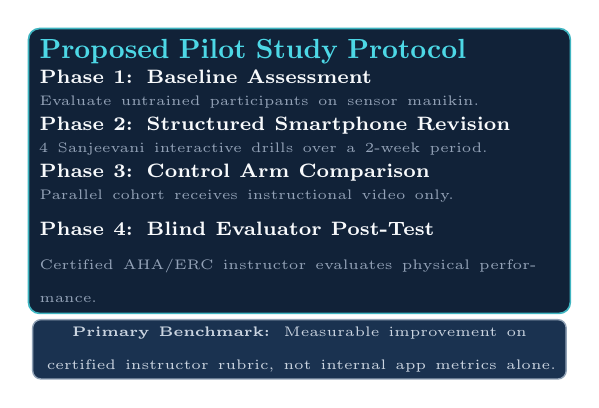
\begin{tikzpicture}
    \node[tealsurface,text width=6.6cm,inner sep=4pt] (pilot) {
      \textbf{\textcolor{TealLight}{Proposed Pilot Study Protocol}}\vspace{1pt}\newline
      \scriptsize
      \textbf{Phase 1: Baseline Assessment}\newline
      \textcolor{TextMuted}{\tiny Evaluate untrained participants on sensor manikin.}\\[1pt]
      \textbf{Phase 2: Structured Smartphone Revision}\newline
      \textcolor{TextMuted}{\tiny 4 Sanjeevani interactive drills over a 2-week period.}\\[1pt]
      \textbf{Phase 3: Control Arm Comparison}\newline
      \textcolor{TextMuted}{\tiny Parallel cohort receives instructional video only.}\\[1pt]
      \textbf{Phase 4: Blind Evaluator Post-Test}\newline
      \textcolor{TextMuted}{\tiny Certified AHA/ERC instructor evaluates physical performance.}
    };

    \node[subtlebox,text width=6.6cm,inner sep=2.5pt,below=0.06cm of pilot,align=center] {
      \centering\tiny\textcolor{TextSub}{\textbf{Primary Benchmark:} Measurable improvement on certified instructor rubric, not internal app metrics alone.}
    };
  \end{tikzpicture}
\end{columns}

\note{Honesty here is critical. Do not present proposals as completed results.
The important distinction: app-internal metrics (counts, completions) are not the same as externally validated learning outcomes.
An expert evaluating the learner's actual technique on a mannequin is the gold standard to aspire to.
Time: ~50 seconds. Transition: "Let me close with the vision this all builds toward."}
\end{frame}

% ── SLIDE 14: CLOSING ──────────────────────────────────────
{
\setbeamertemplate{footline}{}
\begin{frame}[plain]
\begin{tikzpicture}[remember picture,overlay]
  \fill[NavyBg] (current page.south west) rectangle (current page.north east);

  % subtle glowing circle in background (blended with NavyBg)
  \fill[Teal!12!NavyBg] ([xshift=5cm,yshift=0.5cm]current page.center) circle (4.2cm);
  \draw[Teal!25,line width=0.8pt] ([xshift=5cm,yshift=0.5cm]current page.center) circle (4.2cm);

  % Core Closing Vision Box
  \node[anchor=center,tealsurface,text width=13.4cm,inner sep=10pt]
        at ([yshift=0.8cm]current page.center) {
    \centering
    \textcolor{TealLight}{\fontsize{18}{22}\selectfont\bfseries
    ``The goal is not to replace the training room.\\[2pt]
    It is to make practice possible beyond it.''}\\[7pt]
    \small\textcolor{TextSub}{
    Real emergencies do not arrive with advance warning. We cannot place a certified first-aid instructor or a sensor-enabled training manikin beside every citizen whenever they wish to practice. But we can turn the smartphones they already carry into accessible, interactive mirrors for life-saving skills.\\[5pt]
    Sanjeevani bridges the gap between passive awareness and real-world composure --- giving bystanders the opportunity to build muscle memory before the moment someone's life depends on them.}
  };

  % Three closing pillars below (positioned cleanly below box)
  \node[pill] at ([xshift=-4.5cm,yshift=-1.9cm]current page.center)
        {Universal Smartphone Access};
  \node[pill] at ([xshift=0.0cm,yshift=-1.9cm]current page.center)
        {Honest Clinical Engineering};
  \node[pill] at ([xshift=4.5cm,yshift=-1.9cm]current page.center)
        {Verified Muscle Memory};

  \node[anchor=south,text=TextMuted,font=\scriptsize]
        at ([yshift=0.6cm]current page.south)
        {\textbf{\textcolor{TealLight}{SANJEEVANI}} \quad$\cdot$\quad Practice before the moment.};
\end{tikzpicture}
\end{frame}
}

% ── SLIDE 15: SOURCES ──────────────────────────────────────
\begin{frame}{References and Evidence Base}
\framesubtitle{Clinical resuscitation guidelines, empirical literature, and technical frameworks}

\vspace{-0.15cm}
\begin{columns}[T]
\column{0.49\textwidth}
  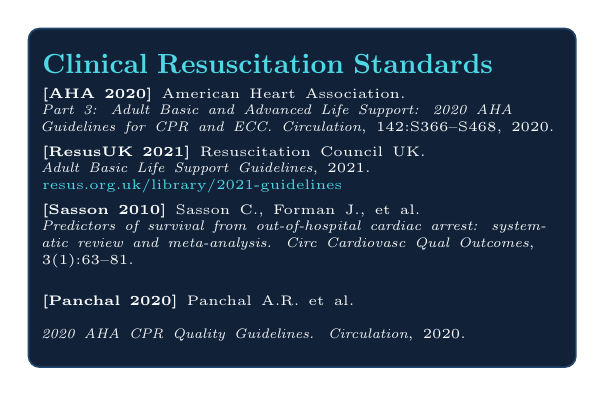
\begin{tikzpicture}
    \node[surface,text width=6.6cm,minimum height=4.3cm] {
      \textbf{\textcolor{TealLight}{Clinical Resuscitation Standards}}\vspace{3pt}\newline
      \tiny
      \textbf{[AHA 2020]} American Heart Association.\newline
      \textit{Part 3: Adult Basic and Advanced Life Support: 2020 AHA Guidelines for CPR and ECC.} \textit{Circulation}, 142:S366--S468, 2020.\\[3pt]
      \textbf{[ResusUK 2021]} Resuscitation Council UK.\newline
      \textit{Adult Basic Life Support Guidelines}, 2021.\newline
      \textcolor{TealLight}{resus.org.uk/library/2021-guidelines}\\[3pt]
      \textbf{[Sasson 2010]} Sasson C., Forman J., et al.\newline
      \textit{Predictors of survival from out-of-hospital cardiac arrest: systematic review and meta-analysis.} \textit{Circ Cardiovasc Qual Outcomes}, 3(1):63--81.\\[3pt]
      \textbf{[Panchal 2020]} Panchal A.R. et al.\newline
      \textit{2020 AHA CPR Quality Guidelines.} \textit{Circulation}, 2020.
    };
  \end{tikzpicture}

\column{0.49\textwidth}
  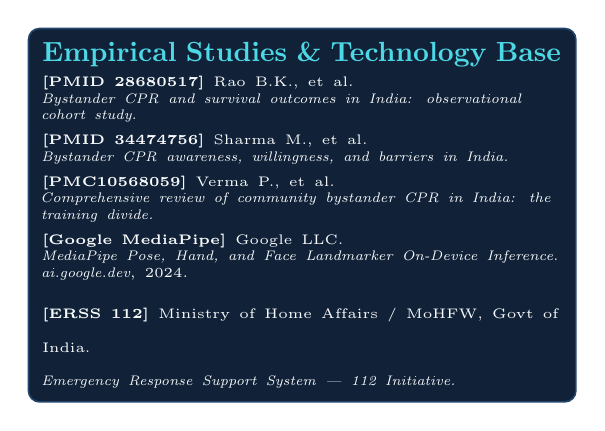
\begin{tikzpicture}
    \node[surface,text width=6.6cm,minimum height=4.3cm] {
      \textbf{\textcolor{TealLight}{Empirical Studies \& Technology Base}}\vspace{3pt}\newline
      \tiny
      \textbf{[PMID 28680517]} Rao B.K., et al.\newline
      \textit{Bystander CPR and survival outcomes in India: observational cohort study.}\\[3pt]
      \textbf{[PMID 34474756]} Sharma M., et al.\newline
      \textit{Bystander CPR awareness, willingness, and barriers in India.}\\[3pt]
      \textbf{[PMC10568059]} Verma P., et al.\newline
      \textit{Comprehensive review of community bystander CPR in India: the training divide.}\\[3pt]
      \textbf{[Google MediaPipe]} Google LLC.\newline
      \textit{MediaPipe Pose, Hand, and Face Landmarker On-Device Inference.} \textit{ai.google.dev}, 2024.\\[3pt]
      \textbf{[ERSS 112]} Ministry of Home Affairs / MoHFW, Govt of India.\newline
      \textit{Emergency Response Support System --- 112 Initiative.}
    };
  \end{tikzpicture}
\end{columns}

\vspace{0.06cm}
\begin{center}

\begin{tikzpicture}
  \node[subtlebox,text width=14.0cm,inner sep=3pt,align=center] {
    \centering\tiny\textcolor{TextMuted}{Manikin pricing and institutional equipment costs vary by supplier and region. All clinical protocols should be validated against local emergency medicine directives.}
  };
\end{tikzpicture}
\end{center}

\end{frame}

\end{document}
